\documentclass{beamer}
\beamertemplatenavigationsymbolsempty
\usecolortheme{beaver}
\setbeamertemplate{blocks}[rounded=true, shadow=true]
\setbeamertemplate{footline}[page number]
%
\usepackage[utf8]{inputenc}
\usepackage[T2A]{fontenc}
\usepackage[russian]{babel}
\usepackage{amssymb,amsfonts,amsmath,mathtext}
\usepackage{subfig}
\usepackage[all]{xy} % xy package for diagrams
\usepackage{array}
\usepackage{multicol}% many columns in slide
\usepackage{hyperref}% urls
\usepackage{hhline}%tables
\usepackage{algorithm}
\usepackage{algpseudocode}
% Your figures are here:
\graphicspath{ {img/} {../figures/} }

%----------------------------------------------------------------------------------------------------------
\title[\hbox to 56mm{Ускоренные безградиентные методы}]{Lab 401: Approximation of direction fields by ODE-Net near the special points for simple ODEs}
\author[Ф.\,А. Хафизов]{Фанис Адикович Хафизов}
\institute{Московский физико-технический институт}
\date{\footnotesize
\par\smallskip\emph{Курс:} Математические методы прогнозирования\par Группа Б05-105
\par\bigskip\small 2024}
%----------------------------------------------------------------------------------------------------------
\begin{document}
%----------------------------------------------------------------------------------------------------------
\begin{frame}
\thispagestyle{empty}
\maketitle
\end{frame}
%-----------------------------------------------------------------------------------------------------

\begin{frame}{Цель работы}
    \textbf{Задача:} Построить направляющее поле и его аппроксимацию с помощью ODE-Net в окрестности особых точек для простых ОДУ (uniform, saddle, center, spiral)
\end{frame}
%-----------------------------------------------------------------------------------------------------

\begin{frame}{Литература}

\begin{itemize}
 \item Ricky T. Q. Chen, Yulia Rubanova, Jesse Bettencourt, David Duvenaud. Neural Ordinary Differential Equations. 2019
 \item Alexander Norcliffe, Cristian Bodnar, Ben Day, Jacob Moss, Pietro Li{\`o}. Neural ODE Processes. 2021
 \item PyTorch Implementation of Differentiable ODE Solvers by Ricky Chen (https://github.com/rtqichen/torchdiffeq)
\end{itemize}

\end{frame}

\begin{frame}{О данных}
    В качестве данных взяты зашумленные траектории решений ОДУ
    $$ \dot{x} = A x, \quad x(0) = x_0. $$
    Траектории для обучения и валидации взяты с началом в разных точках.
\end{frame}

\begin{frame}{Постановка задачи}
    По имеющимся зашумленным участкам траекторий восстановить векторное поле направлений вблизи особых точек.

    Для этого будем делать предсказание ODE-Net траектории решения $x_{pred}^i$ в точках $t^i$, где известно значение $x_{true}^i$, после чего минимизировать MAE:
    $$MAE(x_{pred}, x_{true}) = \frac{1}{l}\sum\limits_{i = 1}^l \|x_{pred} - x_{true}\|_1.$$
\end{frame}

\begin{frame}{Идея ODE-Net}
    Переход от дискретного количества преобразований внутреннего состояния $h$ к непрерывному:
    $$h_{t+1} = h_t + f(h_t, \theta_t) \to \frac{dh(t)}{dt} = f(h(t), t, \theta).$$
    \begin{figure}
     \centering
     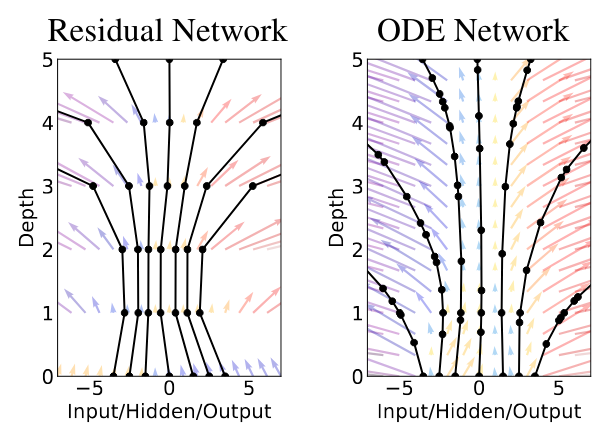
\includegraphics[width=0.7\linewidth]{ODENet}
    \end{figure}
\end{frame}

\begin{frame}{Оптимизация ODE-Net}
 Минимизируется функция
 $$L(x(t_1)) = L\left(x(t_0) + \int\limits_{t_0}^{t_1} f(x(t), t, \theta)\right) \to \min_\theta.$$
 В нашей задаче
 $$L(x(t_k)) = \|x(t_k) - x_{true}(t_k)\|_1,$$
 $f(x(t), t, \theta) = f(x(t), \theta)$ -- двухслойная нейронная сеть, зависимости от времени нет.
\end{frame}

\begin{frame}{Постановка эксперимента}
 Для каждого из 4 рассматриваемых видов особых точек:
 \begin{itemize}
  \item Выписываем матрицу $A \in \mathbb{R}^{2 \times 2}$
  \item Выбираем по 2 стартовых точки для train $x^1(0), x^2(0)$ и по 1 для test $x_{test}(0)$.
  \item Находим численные решения дифференциального уравнения $x^1(t), x^2(t), x_{test}(t)$ в точках $t_i$.
  \item Берем подпоследовательность в одной из траекторий, зашумляем ее, получаем предсказание $x_{pred}(t)$
  \item Считаем MAE, обновляем параметры сети
  \item Рисуем фазовый портрет для всех траекторий и поле направлений
 \end{itemize}
\end{frame}

\begin{frame}{Эксперимент}
\begin{figure}
 \centering
 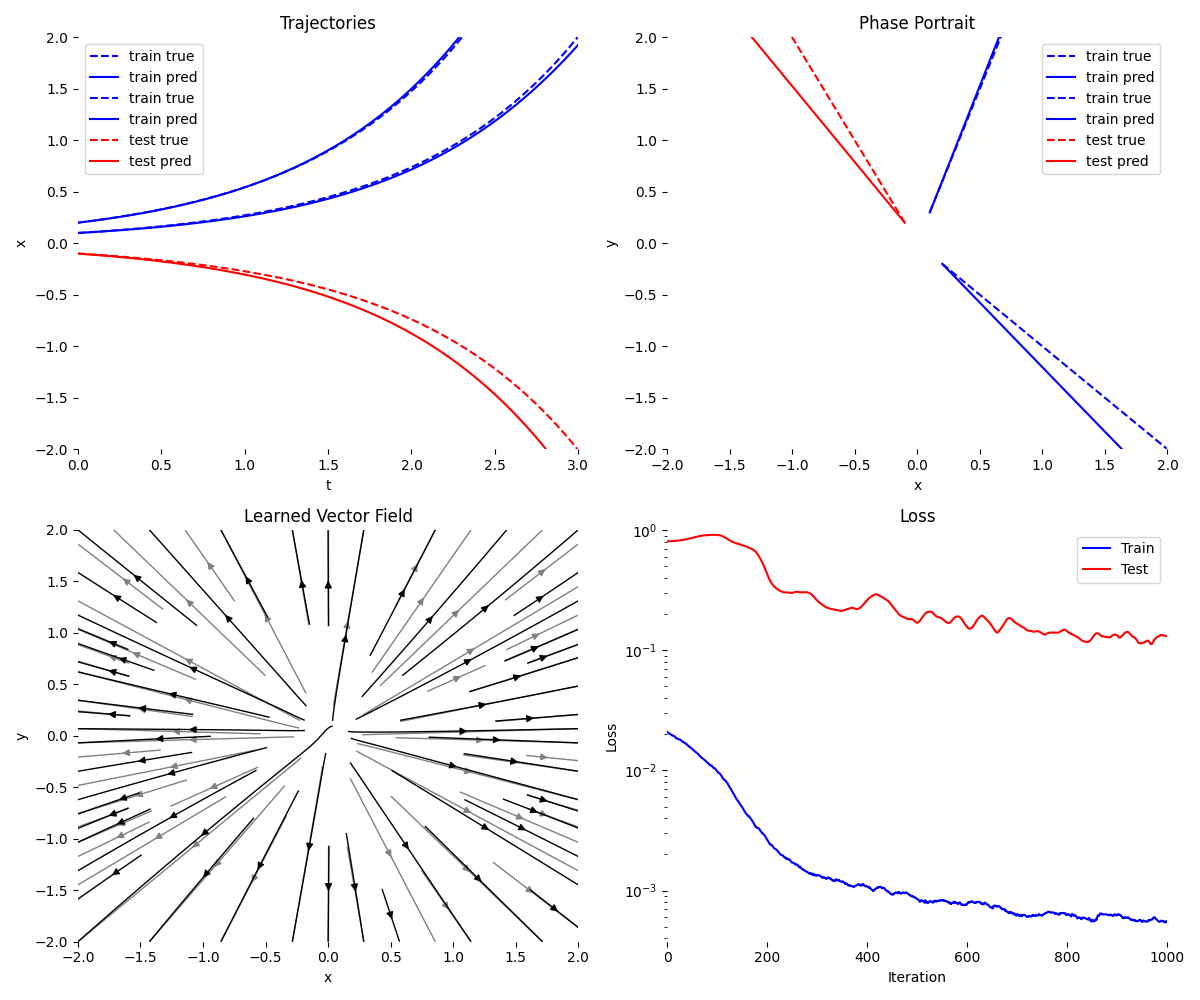
\includegraphics[width=0.8\linewidth]{uniform-0.0}
 \caption{Uniform. Без шума}
\end{figure}
\end{frame}

\begin{frame}{Эксперимент}
\begin{figure}
 \centering
 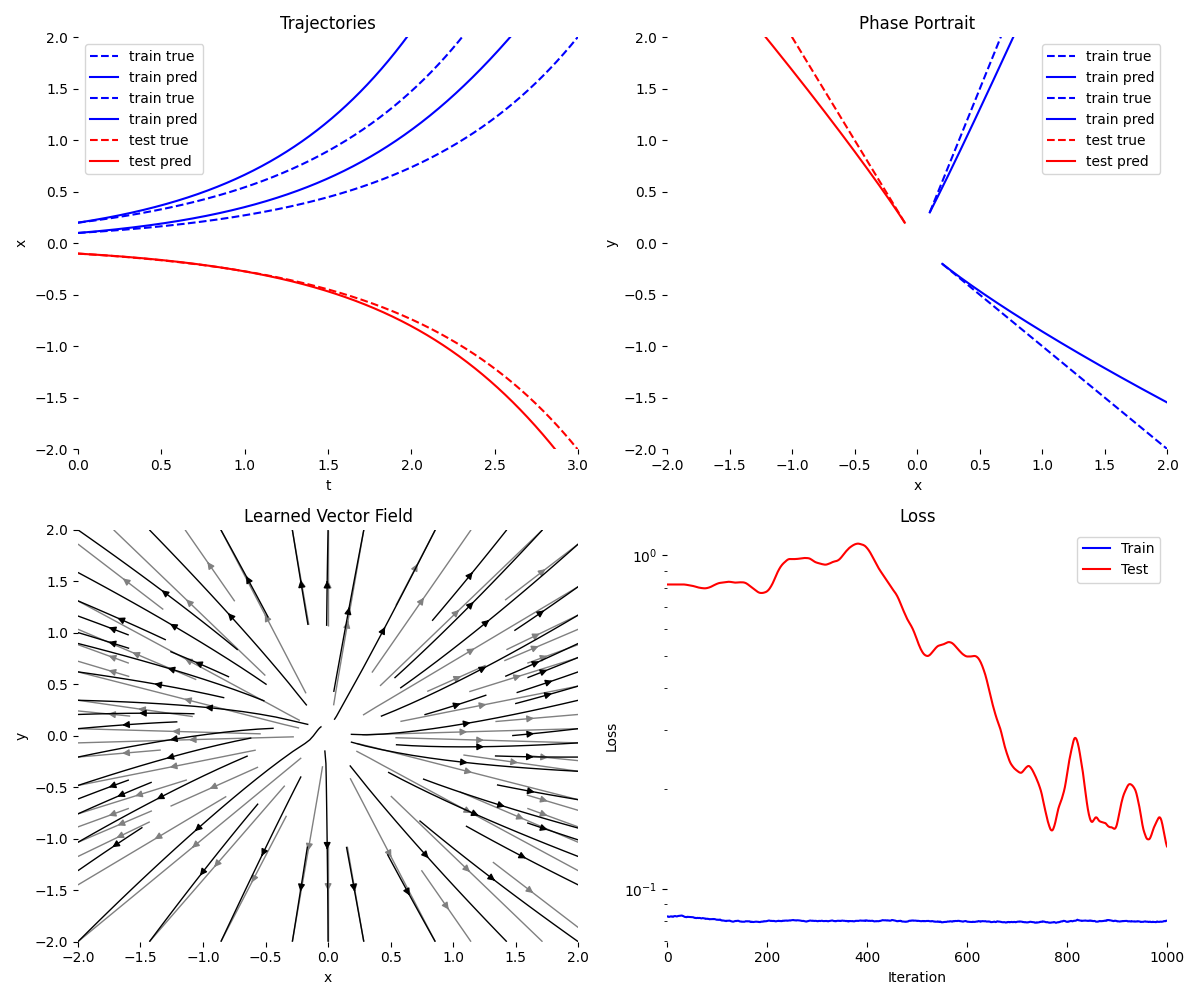
\includegraphics[width=0.8\linewidth]{uniform-0.1}
 \caption{Uniform. Шум из $N(0, 0.1)$}
\end{figure}
\end{frame}

\begin{frame}{Эксперимент}
\begin{figure}
 \centering
 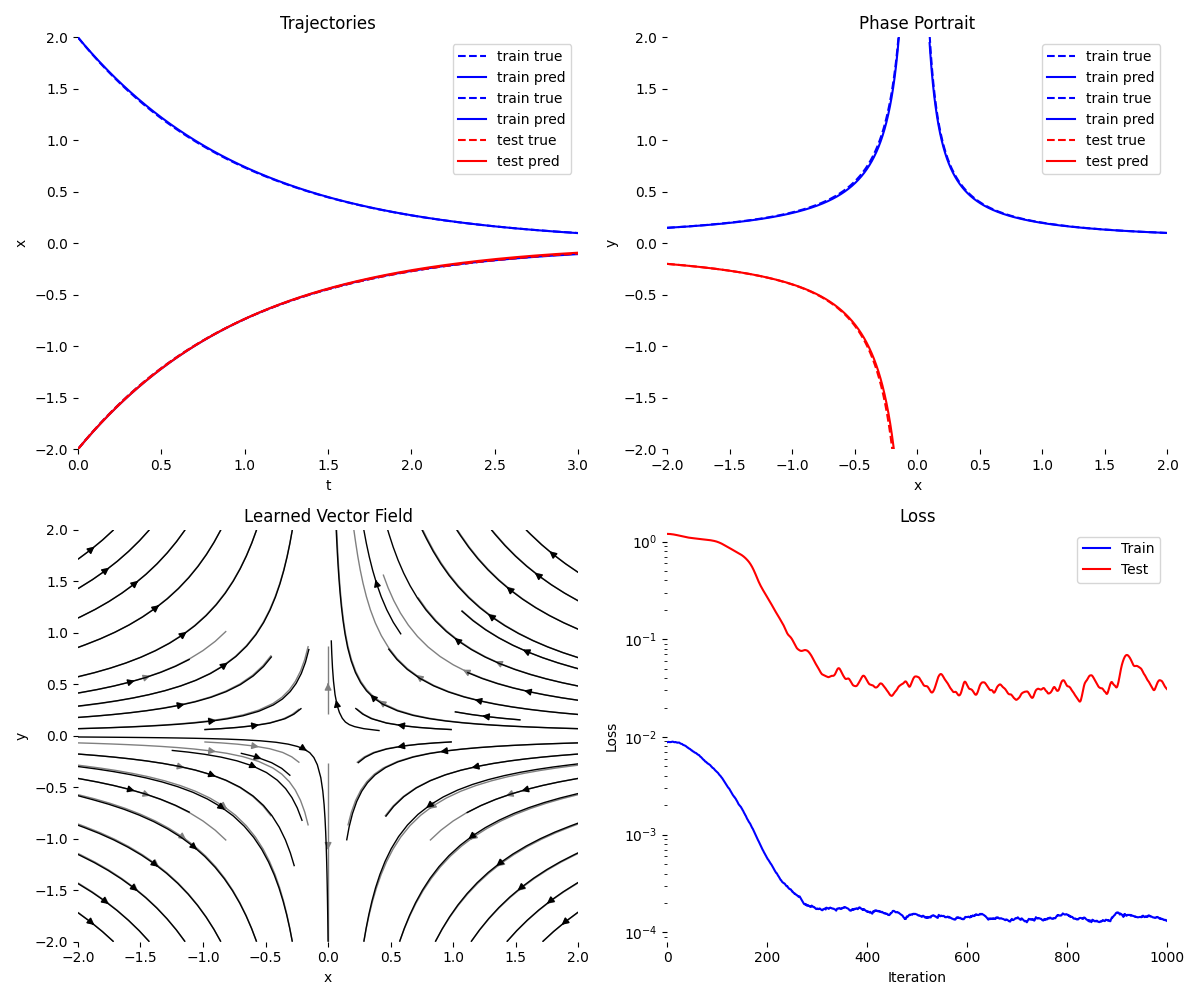
\includegraphics[width=0.8\linewidth]{saddle-0.0}
 \caption{Saddle. Без шума}
\end{figure}
\end{frame}

\begin{frame}{Эксперимент}
\begin{figure}
 \centering
 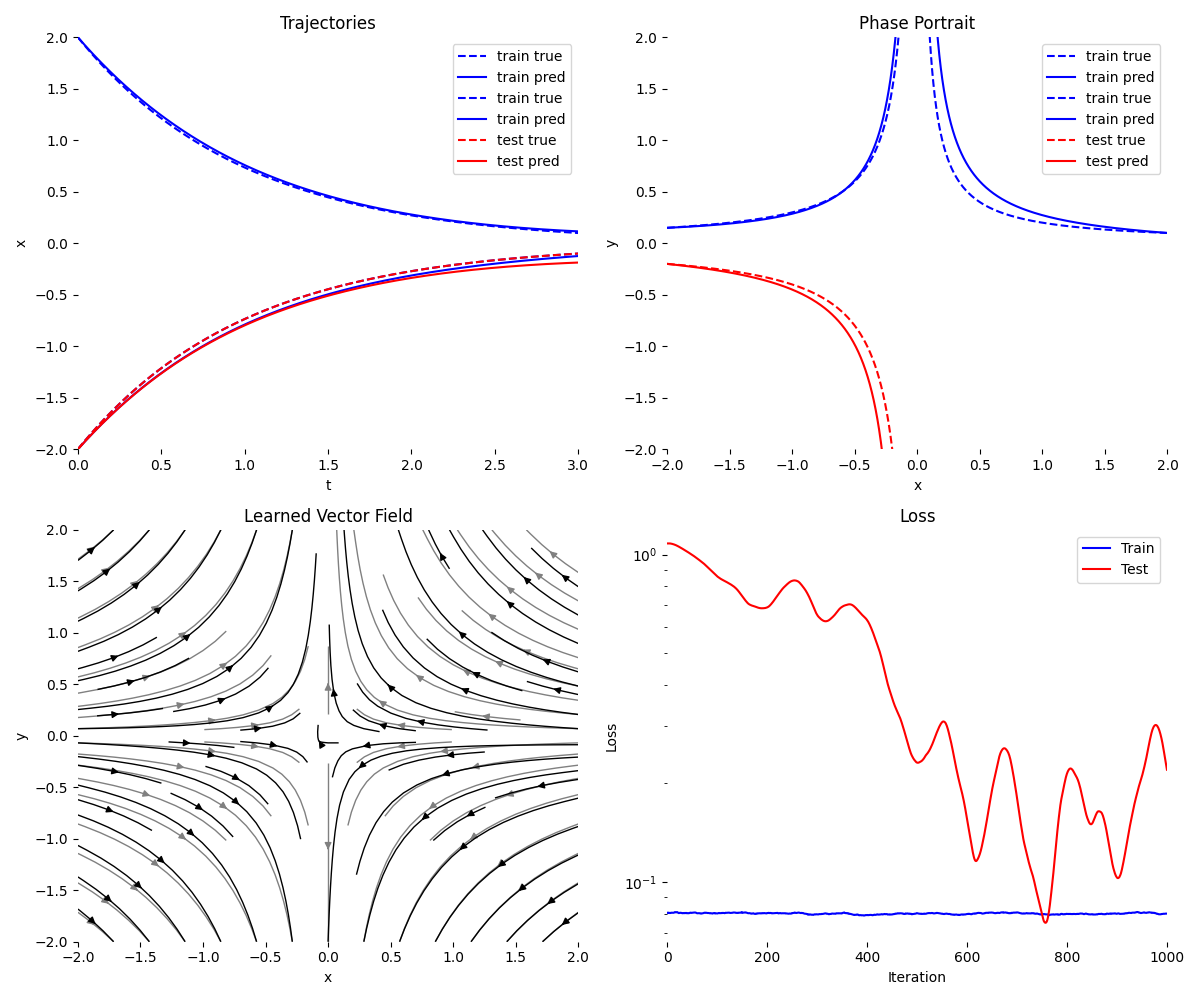
\includegraphics[width=0.8\linewidth]{saddle-0.1}
 \caption{Saddle. Шум из $N(0, 0.1)$}
\end{figure}
\end{frame}

\begin{frame}{Эксперимент}
\begin{figure}
 \centering
 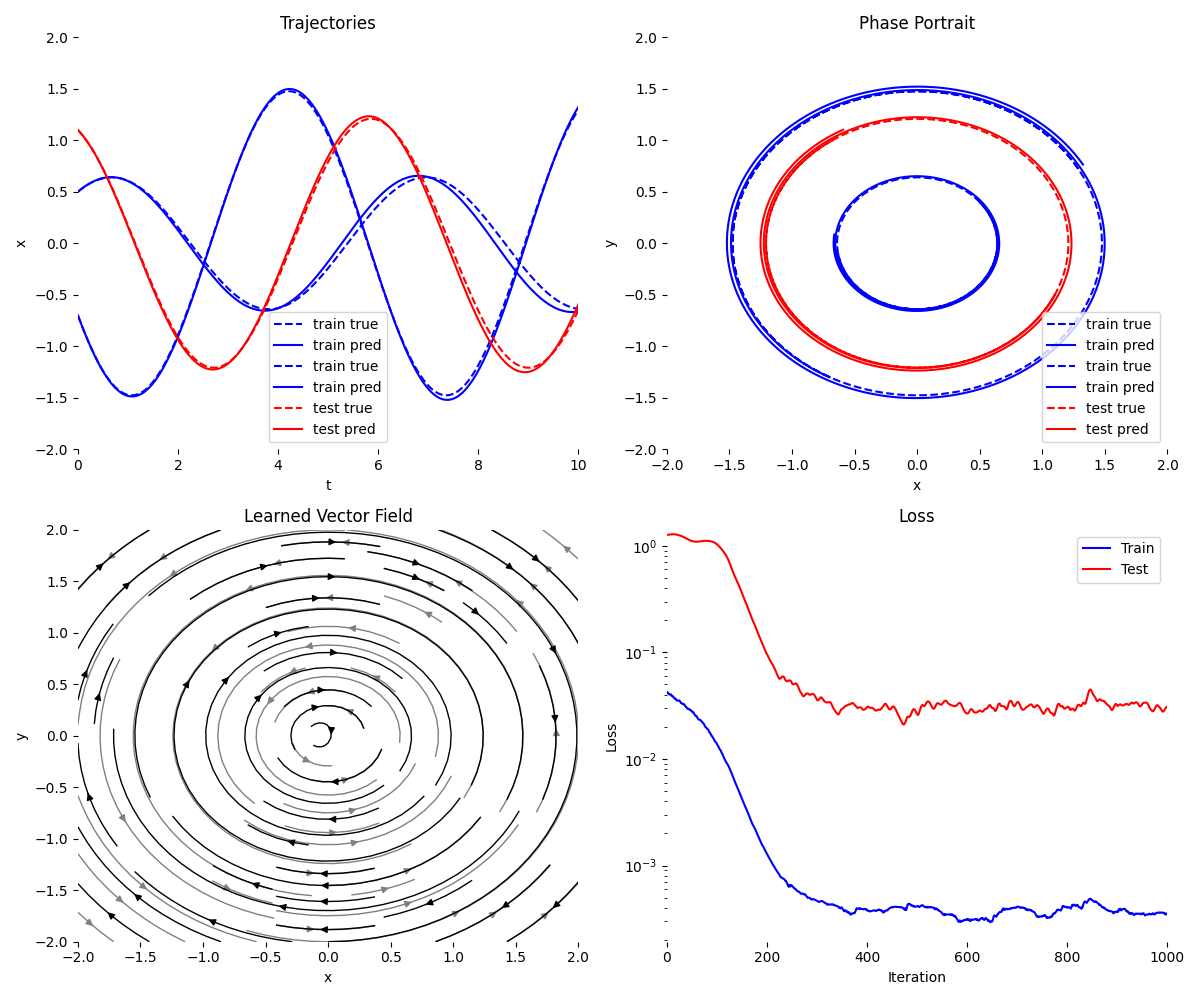
\includegraphics[width=0.8\linewidth]{center-0.0}
 \caption{Center. Без шума}
\end{figure}
\end{frame}

\begin{frame}{Эксперимент}
\begin{figure}
 \centering
 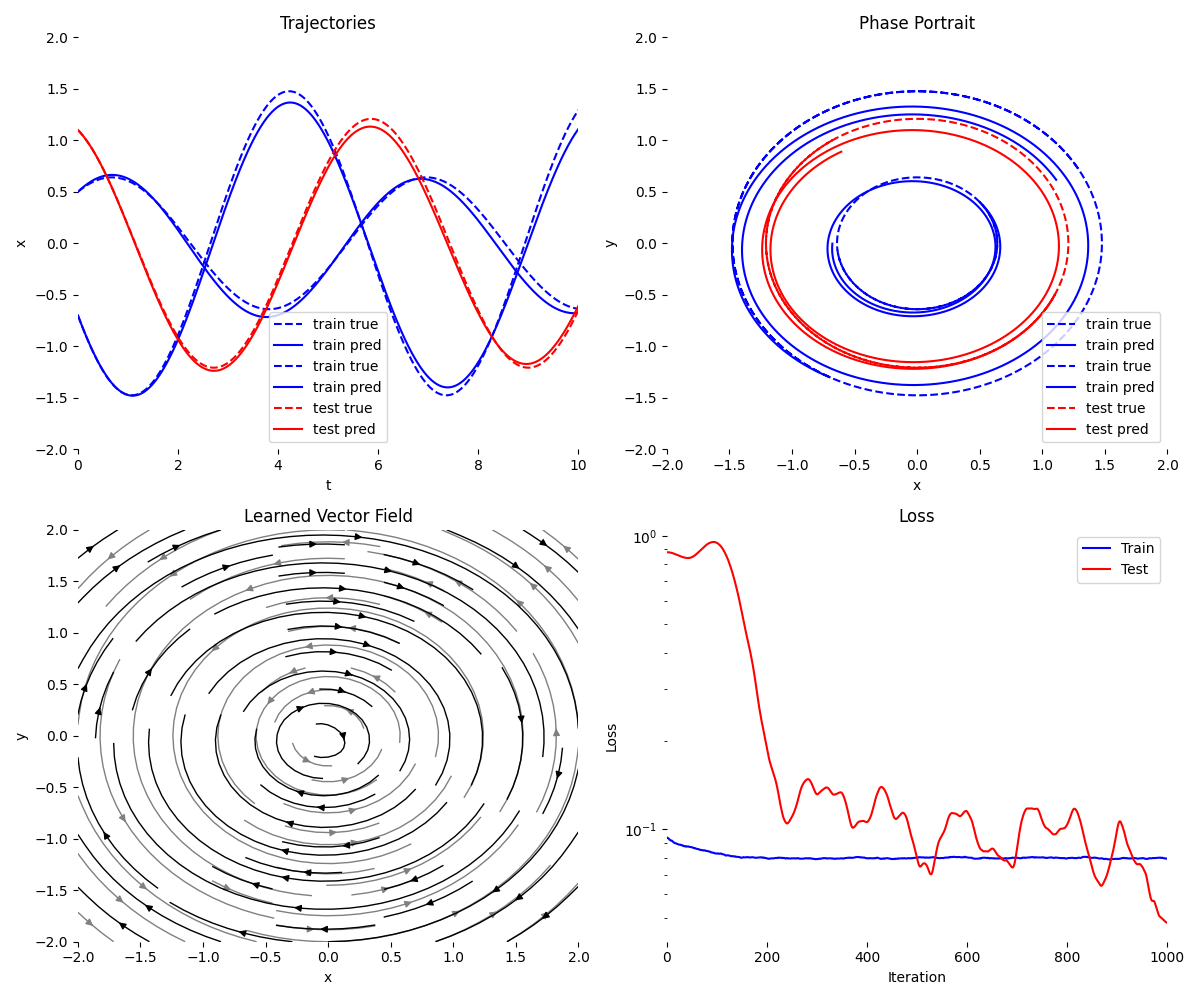
\includegraphics[width=0.8\linewidth]{center-0.1}
 \caption{Center. Шум из $N(0, 0.1)$}
\end{figure}
\end{frame}

\begin{frame}{Эксперимент}
\begin{figure}
 \centering
 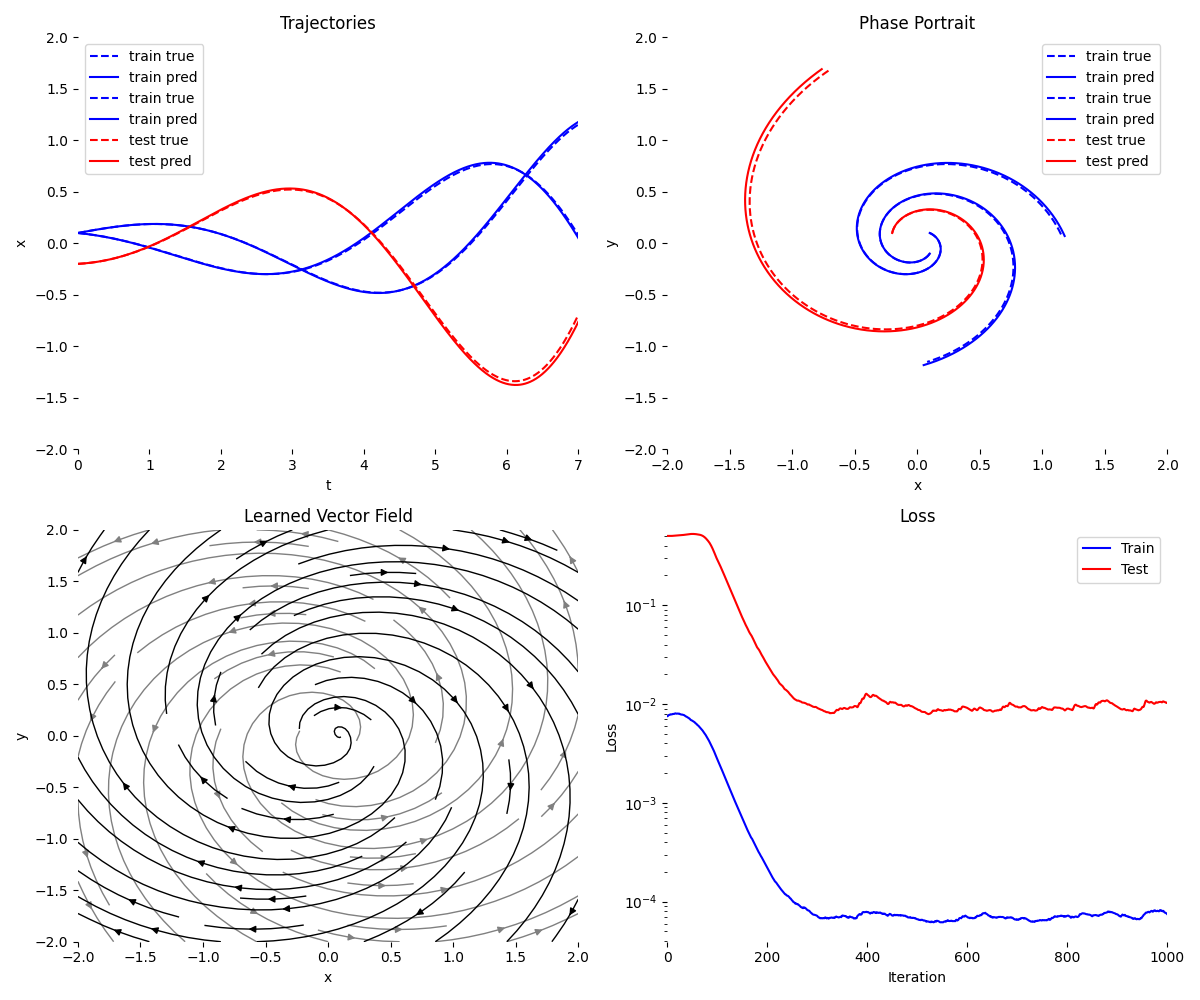
\includegraphics[width=0.8\linewidth]{spiral-0.0}
 \caption{Spiral. Без шума}
\end{figure}
\end{frame}

\begin{frame}{Эксперимент}
\begin{figure}
 \centering
 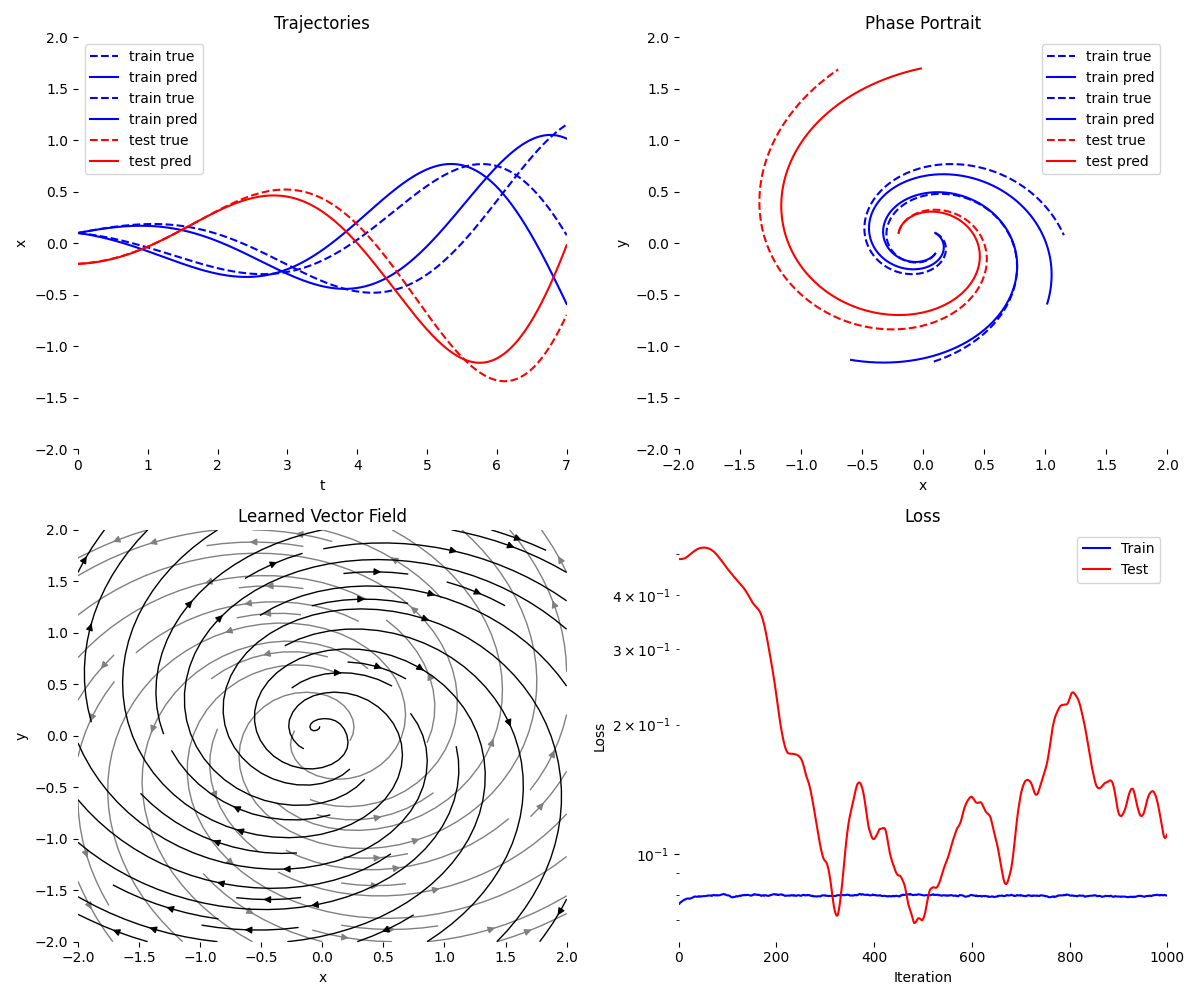
\includegraphics[width=0.8\linewidth]{spiral-0.1}
 \caption{Spiral. Шум из $N(0, 0.1)$}
\end{figure}
\end{frame}

\begin{frame}{Выводы}
 \begin{itemize}
  \item Обученная модель достаточно точно восстанавливает векторное поле направлений, даже при наличии шума в данных.
  \item Выбор двух различных траекторий для обучения позволяет более точно восстанавливать сложные траектории, такие как saddle и uniform.
  \item На самом деле выбранная модель избыточна для нашей задачи, ведь обученное преобразование приближает $A: x \to Ax$.
 \end{itemize}
\end{frame}

\begin{frame}{Будущая работа}
 \begin{itemize}
  \item Научиться решать нелинейные системы уравнений, то есть, вида
  $$\dot{x} = g(x),$$
  где $g(x)$ не обязательно линейная функция.
 \end{itemize}
\end{frame}

\end{document}
